% Created by tikzDevice version 0.11 on 2018-04-28 12:09:13
% !TEX encoding = UTF-8 Unicode
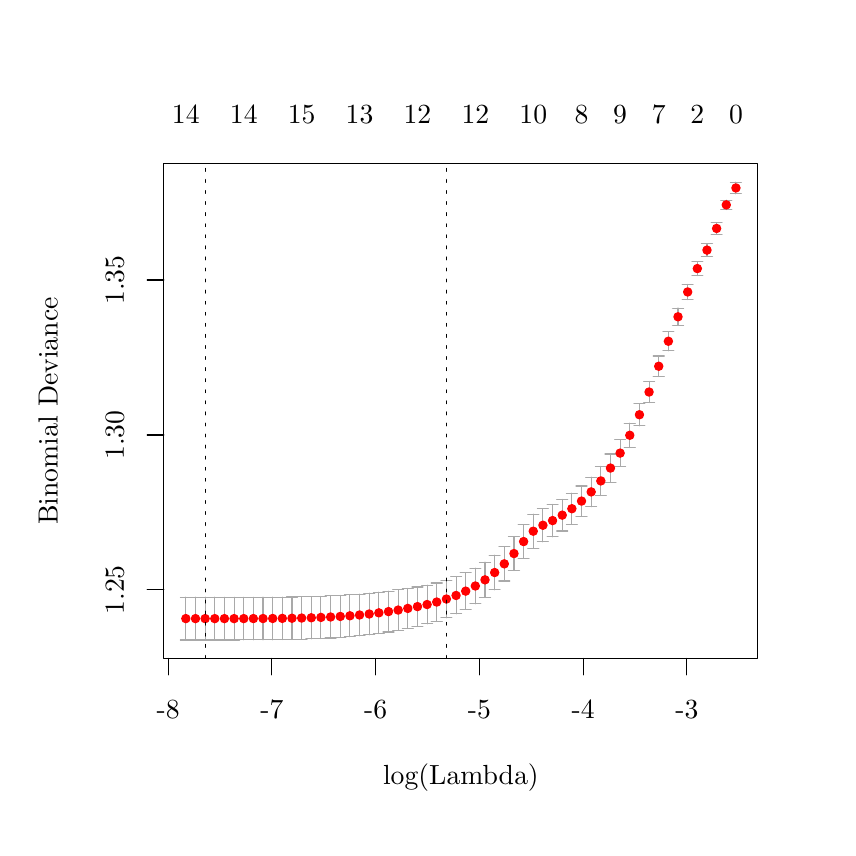
\begin{tikzpicture}[x=1pt,y=1pt]
\definecolor{fillColor}{RGB}{255,255,255}
\path[use as bounding box,fill=fillColor,fill opacity=0.00] (0,0) rectangle (289.08,289.08);
\begin{scope}
\path[clip] (  0.00,  0.00) rectangle (289.08,289.08);
\definecolor{drawColor}{RGB}{0,0,0}

\path[draw=drawColor,line width= 0.4pt,line join=round,line cap=round] ( 50.77, 61.20) -- (238.19, 61.20);

\path[draw=drawColor,line width= 0.4pt,line join=round,line cap=round] ( 50.77, 61.20) -- ( 50.77, 55.20);

\path[draw=drawColor,line width= 0.4pt,line join=round,line cap=round] ( 88.25, 61.20) -- ( 88.25, 55.20);

\path[draw=drawColor,line width= 0.4pt,line join=round,line cap=round] (125.74, 61.20) -- (125.74, 55.20);

\path[draw=drawColor,line width= 0.4pt,line join=round,line cap=round] (163.22, 61.20) -- (163.22, 55.20);

\path[draw=drawColor,line width= 0.4pt,line join=round,line cap=round] (200.70, 61.20) -- (200.70, 55.20);

\path[draw=drawColor,line width= 0.4pt,line join=round,line cap=round] (238.19, 61.20) -- (238.19, 55.20);

\node[text=drawColor,anchor=base,inner sep=0pt, outer sep=0pt, scale=  1.00] at ( 50.77, 39.60) {-8};

\node[text=drawColor,anchor=base,inner sep=0pt, outer sep=0pt, scale=  1.00] at ( 88.25, 39.60) {-7};

\node[text=drawColor,anchor=base,inner sep=0pt, outer sep=0pt, scale=  1.00] at (125.74, 39.60) {-6};

\node[text=drawColor,anchor=base,inner sep=0pt, outer sep=0pt, scale=  1.00] at (163.22, 39.60) {-5};

\node[text=drawColor,anchor=base,inner sep=0pt, outer sep=0pt, scale=  1.00] at (200.70, 39.60) {-4};

\node[text=drawColor,anchor=base,inner sep=0pt, outer sep=0pt, scale=  1.00] at (238.19, 39.60) {-3};

\path[draw=drawColor,line width= 0.4pt,line join=round,line cap=round] ( 49.20, 85.92) -- ( 49.20,197.88);

\path[draw=drawColor,line width= 0.4pt,line join=round,line cap=round] ( 49.20, 85.92) -- ( 43.20, 85.92);

\path[draw=drawColor,line width= 0.4pt,line join=round,line cap=round] ( 49.20,141.90) -- ( 43.20,141.90);

\path[draw=drawColor,line width= 0.4pt,line join=round,line cap=round] ( 49.20,197.88) -- ( 43.20,197.88);

\node[text=drawColor,rotate= 90.00,anchor=base,inner sep=0pt, outer sep=0pt, scale=  1.00] at ( 34.80, 85.92) {1.25};

\node[text=drawColor,rotate= 90.00,anchor=base,inner sep=0pt, outer sep=0pt, scale=  1.00] at ( 34.80,141.90) {1.30};

\node[text=drawColor,rotate= 90.00,anchor=base,inner sep=0pt, outer sep=0pt, scale=  1.00] at ( 34.80,197.88) {1.35};

\path[draw=drawColor,line width= 0.4pt,line join=round,line cap=round] ( 49.20, 61.20) --
	(263.88, 61.20) --
	(263.88,239.88) --
	( 49.20,239.88) --
	( 49.20, 61.20);
\end{scope}
\begin{scope}
\path[clip] (  0.00,  0.00) rectangle (289.08,289.08);
\definecolor{drawColor}{RGB}{0,0,0}

\node[text=drawColor,anchor=base,inner sep=0pt, outer sep=0pt, scale=  1.00] at (156.54, 15.60) {log(Lambda)};

\node[text=drawColor,rotate= 90.00,anchor=base,inner sep=0pt, outer sep=0pt, scale=  1.00] at ( 10.80,150.54) {Binomial Deviance};
\end{scope}
\begin{scope}
\path[clip] ( 49.20, 61.20) rectangle (263.88,239.88);
\definecolor{drawColor}{RGB}{169,169,169}

\path[draw=drawColor,line width= 0.4pt,line join=round,line cap=round] (255.93,233.26) -- (255.93,229.06);

\path[draw=drawColor,line width= 0.4pt,line join=round,line cap=round] (252.44,226.74) -- (252.44,223.35);

\path[draw=drawColor,line width= 0.4pt,line join=round,line cap=round] (248.95,218.56) -- (248.95,214.50);

\path[draw=drawColor,line width= 0.4pt,line join=round,line cap=round] (245.47,210.99) -- (245.47,206.41);

\path[draw=drawColor,line width= 0.4pt,line join=round,line cap=round] (241.98,204.56) -- (241.98,199.49);

\path[draw=drawColor,line width= 0.4pt,line join=round,line cap=round] (238.49,196.33) -- (238.49,190.84);

\path[draw=drawColor,line width= 0.4pt,line join=round,line cap=round] (235.00,187.74) -- (235.00,181.46);

\path[draw=drawColor,line width= 0.4pt,line join=round,line cap=round] (231.52,179.23) -- (231.52,172.31);

\path[draw=drawColor,line width= 0.4pt,line join=round,line cap=round] (228.03,170.42) -- (228.03,163.03);

\path[draw=drawColor,line width= 0.4pt,line join=round,line cap=round] (224.54,161.26) -- (224.54,153.59);

\path[draw=drawColor,line width= 0.4pt,line join=round,line cap=round] (221.06,153.23) -- (221.06,145.19);

\path[draw=drawColor,line width= 0.4pt,line join=round,line cap=round] (217.57,146.20) -- (217.57,137.38);

\path[draw=drawColor,line width= 0.4pt,line join=round,line cap=round] (214.08,140.14) -- (214.08,130.57);

\path[draw=drawColor,line width= 0.4pt,line join=round,line cap=round] (210.59,135.04) -- (210.59,124.83);

\path[draw=drawColor,line width= 0.4pt,line join=round,line cap=round] (207.11,130.58) -- (207.11,120.02);

\path[draw=drawColor,line width= 0.4pt,line join=round,line cap=round] (203.62,126.68) -- (203.62,115.98);

\path[draw=drawColor,line width= 0.4pt,line join=round,line cap=round] (200.13,123.47) -- (200.13,112.56);

\path[draw=drawColor,line width= 0.4pt,line join=round,line cap=round] (196.64,120.85) -- (196.64,109.67);

\path[draw=drawColor,line width= 0.4pt,line join=round,line cap=round] (193.16,118.65) -- (193.16,107.21);

\path[draw=drawColor,line width= 0.4pt,line join=round,line cap=round] (189.67,116.80) -- (189.67,105.11);

\path[draw=drawColor,line width= 0.4pt,line join=round,line cap=round] (186.18,115.25) -- (186.18,103.31);

\path[draw=drawColor,line width= 0.4pt,line join=round,line cap=round] (182.69,113.31) -- (182.69,100.96);

\path[draw=drawColor,line width= 0.4pt,line join=round,line cap=round] (179.21,109.47) -- (179.21, 97.29);

\path[draw=drawColor,line width= 0.4pt,line join=round,line cap=round] (175.72,105.19) -- (175.72, 92.92);

\path[draw=drawColor,line width= 0.4pt,line join=round,line cap=round] (172.23,101.53) -- (172.23, 89.13);

\path[draw=drawColor,line width= 0.4pt,line join=round,line cap=round] (168.75, 98.47) -- (168.75, 85.92);

\path[draw=drawColor,line width= 0.4pt,line join=round,line cap=round] (165.26, 95.92) -- (165.26, 83.18);

\path[draw=drawColor,line width= 0.4pt,line join=round,line cap=round] (161.77, 93.80) -- (161.77, 80.85);

\path[draw=drawColor,line width= 0.4pt,line join=round,line cap=round] (158.28, 92.05) -- (158.28, 78.88);

\path[draw=drawColor,line width= 0.4pt,line join=round,line cap=round] (154.80, 90.60) -- (154.80, 77.23);

\path[draw=drawColor,line width= 0.4pt,line join=round,line cap=round] (151.31, 89.40) -- (151.31, 75.83);

\path[draw=drawColor,line width= 0.4pt,line join=round,line cap=round] (147.82, 88.42) -- (147.82, 74.64);

\path[draw=drawColor,line width= 0.4pt,line join=round,line cap=round] (144.33, 87.62) -- (144.33, 73.64);

\path[draw=drawColor,line width= 0.4pt,line join=round,line cap=round] (140.85, 86.97) -- (140.85, 72.80);

\path[draw=drawColor,line width= 0.4pt,line join=round,line cap=round] (137.36, 86.43) -- (137.36, 72.04);

\path[draw=drawColor,line width= 0.4pt,line join=round,line cap=round] (133.87, 85.91) -- (133.87, 71.34);

\path[draw=drawColor,line width= 0.4pt,line join=round,line cap=round] (130.39, 85.46) -- (130.39, 70.70);

\path[draw=drawColor,line width= 0.4pt,line join=round,line cap=round] (126.90, 85.10) -- (126.90, 70.17);

\path[draw=drawColor,line width= 0.4pt,line join=round,line cap=round] (123.41, 84.71) -- (123.41, 69.71);

\path[draw=drawColor,line width= 0.4pt,line join=round,line cap=round] (119.92, 84.38) -- (119.92, 69.32);

\path[draw=drawColor,line width= 0.4pt,line join=round,line cap=round] (116.44, 84.11) -- (116.44, 69.00);

\path[draw=drawColor,line width= 0.4pt,line join=round,line cap=round] (112.95, 83.90) -- (112.95, 68.74);

\path[draw=drawColor,line width= 0.4pt,line join=round,line cap=round] (109.46, 83.74) -- (109.46, 68.53);

\path[draw=drawColor,line width= 0.4pt,line join=round,line cap=round] (105.97, 83.60) -- (105.97, 68.35);

\path[draw=drawColor,line width= 0.4pt,line join=round,line cap=round] (102.49, 83.50) -- (102.49, 68.21);

\path[draw=drawColor,line width= 0.4pt,line join=round,line cap=round] ( 99.00, 83.41) -- ( 99.00, 68.09);

\path[draw=drawColor,line width= 0.4pt,line join=round,line cap=round] ( 95.51, 83.35) -- ( 95.51, 68.01);

\path[draw=drawColor,line width= 0.4pt,line join=round,line cap=round] ( 92.02, 83.31) -- ( 92.02, 67.95);

\path[draw=drawColor,line width= 0.4pt,line join=round,line cap=round] ( 88.54, 83.28) -- ( 88.54, 67.91);

\path[draw=drawColor,line width= 0.4pt,line join=round,line cap=round] ( 85.05, 83.26) -- ( 85.05, 67.88);

\path[draw=drawColor,line width= 0.4pt,line join=round,line cap=round] ( 81.56, 83.25) -- ( 81.56, 67.86);

\path[draw=drawColor,line width= 0.4pt,line join=round,line cap=round] ( 78.08, 83.25) -- ( 78.08, 67.84);

\path[draw=drawColor,line width= 0.4pt,line join=round,line cap=round] ( 74.59, 83.25) -- ( 74.59, 67.83);

\path[draw=drawColor,line width= 0.4pt,line join=round,line cap=round] ( 71.10, 83.25) -- ( 71.10, 67.83);

\path[draw=drawColor,line width= 0.4pt,line join=round,line cap=round] ( 67.61, 83.26) -- ( 67.61, 67.82);

\path[draw=drawColor,line width= 0.4pt,line join=round,line cap=round] ( 64.13, 83.26) -- ( 64.13, 67.82);

\path[draw=drawColor,line width= 0.4pt,line join=round,line cap=round] ( 60.64, 83.27) -- ( 60.64, 67.82);

\path[draw=drawColor,line width= 0.4pt,line join=round,line cap=round] ( 57.15, 83.27) -- ( 57.15, 67.82);

\path[draw=drawColor,line width= 0.4pt,line join=round,line cap=round] (253.94,233.26) -- (257.92,233.26);

\path[draw=drawColor,line width= 0.4pt,line join=round,line cap=round] (250.45,226.74) -- (254.43,226.74);

\path[draw=drawColor,line width= 0.4pt,line join=round,line cap=round] (246.97,218.56) -- (250.94,218.56);

\path[draw=drawColor,line width= 0.4pt,line join=round,line cap=round] (243.48,210.99) -- (247.45,210.99);

\path[draw=drawColor,line width= 0.4pt,line join=round,line cap=round] (239.99,204.56) -- (243.97,204.56);

\path[draw=drawColor,line width= 0.4pt,line join=round,line cap=round] (236.50,196.33) -- (240.48,196.33);

\path[draw=drawColor,line width= 0.4pt,line join=round,line cap=round] (233.02,187.74) -- (236.99,187.74);

\path[draw=drawColor,line width= 0.4pt,line join=round,line cap=round] (229.53,179.23) -- (233.51,179.23);

\path[draw=drawColor,line width= 0.4pt,line join=round,line cap=round] (226.04,170.42) -- (230.02,170.42);

\path[draw=drawColor,line width= 0.4pt,line join=round,line cap=round] (222.56,161.26) -- (226.53,161.26);

\path[draw=drawColor,line width= 0.4pt,line join=round,line cap=round] (219.07,153.23) -- (223.04,153.23);

\path[draw=drawColor,line width= 0.4pt,line join=round,line cap=round] (215.58,146.20) -- (219.56,146.20);

\path[draw=drawColor,line width= 0.4pt,line join=round,line cap=round] (212.09,140.14) -- (216.07,140.14);

\path[draw=drawColor,line width= 0.4pt,line join=round,line cap=round] (208.61,135.04) -- (212.58,135.04);

\path[draw=drawColor,line width= 0.4pt,line join=round,line cap=round] (205.12,130.58) -- (209.09,130.58);

\path[draw=drawColor,line width= 0.4pt,line join=round,line cap=round] (201.63,126.68) -- (205.61,126.68);

\path[draw=drawColor,line width= 0.4pt,line join=round,line cap=round] (198.14,123.47) -- (202.12,123.47);

\path[draw=drawColor,line width= 0.4pt,line join=round,line cap=round] (194.66,120.85) -- (198.63,120.85);

\path[draw=drawColor,line width= 0.4pt,line join=round,line cap=round] (191.17,118.65) -- (195.14,118.65);

\path[draw=drawColor,line width= 0.4pt,line join=round,line cap=round] (187.68,116.80) -- (191.66,116.80);

\path[draw=drawColor,line width= 0.4pt,line join=round,line cap=round] (184.19,115.25) -- (188.17,115.25);

\path[draw=drawColor,line width= 0.4pt,line join=round,line cap=round] (180.71,113.31) -- (184.68,113.31);

\path[draw=drawColor,line width= 0.4pt,line join=round,line cap=round] (177.22,109.47) -- (181.20,109.47);

\path[draw=drawColor,line width= 0.4pt,line join=round,line cap=round] (173.73,105.19) -- (177.71,105.19);

\path[draw=drawColor,line width= 0.4pt,line join=round,line cap=round] (170.25,101.53) -- (174.22,101.53);

\path[draw=drawColor,line width= 0.4pt,line join=round,line cap=round] (166.76, 98.47) -- (170.73, 98.47);

\path[draw=drawColor,line width= 0.4pt,line join=round,line cap=round] (163.27, 95.92) -- (167.25, 95.92);

\path[draw=drawColor,line width= 0.4pt,line join=round,line cap=round] (159.78, 93.80) -- (163.76, 93.80);

\path[draw=drawColor,line width= 0.4pt,line join=round,line cap=round] (156.30, 92.05) -- (160.27, 92.05);

\path[draw=drawColor,line width= 0.4pt,line join=round,line cap=round] (152.81, 90.60) -- (156.78, 90.60);

\path[draw=drawColor,line width= 0.4pt,line join=round,line cap=round] (149.32, 89.40) -- (153.30, 89.40);

\path[draw=drawColor,line width= 0.4pt,line join=round,line cap=round] (145.83, 88.42) -- (149.81, 88.42);

\path[draw=drawColor,line width= 0.4pt,line join=round,line cap=round] (142.35, 87.62) -- (146.32, 87.62);

\path[draw=drawColor,line width= 0.4pt,line join=round,line cap=round] (138.86, 86.97) -- (142.83, 86.97);

\path[draw=drawColor,line width= 0.4pt,line join=round,line cap=round] (135.37, 86.43) -- (139.35, 86.43);

\path[draw=drawColor,line width= 0.4pt,line join=round,line cap=round] (131.88, 85.91) -- (135.86, 85.91);

\path[draw=drawColor,line width= 0.4pt,line join=round,line cap=round] (128.40, 85.46) -- (132.37, 85.46);

\path[draw=drawColor,line width= 0.4pt,line join=round,line cap=round] (124.91, 85.10) -- (128.89, 85.10);

\path[draw=drawColor,line width= 0.4pt,line join=round,line cap=round] (121.42, 84.71) -- (125.40, 84.71);

\path[draw=drawColor,line width= 0.4pt,line join=round,line cap=round] (117.94, 84.38) -- (121.91, 84.38);

\path[draw=drawColor,line width= 0.4pt,line join=round,line cap=round] (114.45, 84.11) -- (118.42, 84.11);

\path[draw=drawColor,line width= 0.4pt,line join=round,line cap=round] (110.96, 83.90) -- (114.94, 83.90);

\path[draw=drawColor,line width= 0.4pt,line join=round,line cap=round] (107.47, 83.74) -- (111.45, 83.74);

\path[draw=drawColor,line width= 0.4pt,line join=round,line cap=round] (103.99, 83.60) -- (107.96, 83.60);

\path[draw=drawColor,line width= 0.4pt,line join=round,line cap=round] (100.50, 83.50) -- (104.47, 83.50);

\path[draw=drawColor,line width= 0.4pt,line join=round,line cap=round] ( 97.01, 83.41) -- (100.99, 83.41);

\path[draw=drawColor,line width= 0.4pt,line join=round,line cap=round] ( 93.52, 83.35) -- ( 97.50, 83.35);

\path[draw=drawColor,line width= 0.4pt,line join=round,line cap=round] ( 90.04, 83.31) -- ( 94.01, 83.31);

\path[draw=drawColor,line width= 0.4pt,line join=round,line cap=round] ( 86.55, 83.28) -- ( 90.52, 83.28);

\path[draw=drawColor,line width= 0.4pt,line join=round,line cap=round] ( 83.06, 83.26) -- ( 87.04, 83.26);

\path[draw=drawColor,line width= 0.4pt,line join=round,line cap=round] ( 79.57, 83.25) -- ( 83.55, 83.25);

\path[draw=drawColor,line width= 0.4pt,line join=round,line cap=round] ( 76.09, 83.25) -- ( 80.06, 83.25);

\path[draw=drawColor,line width= 0.4pt,line join=round,line cap=round] ( 72.60, 83.25) -- ( 76.58, 83.25);

\path[draw=drawColor,line width= 0.4pt,line join=round,line cap=round] ( 69.11, 83.25) -- ( 73.09, 83.25);

\path[draw=drawColor,line width= 0.4pt,line join=round,line cap=round] ( 65.63, 83.26) -- ( 69.60, 83.26);

\path[draw=drawColor,line width= 0.4pt,line join=round,line cap=round] ( 62.14, 83.26) -- ( 66.11, 83.26);

\path[draw=drawColor,line width= 0.4pt,line join=round,line cap=round] ( 58.65, 83.27) -- ( 62.63, 83.27);

\path[draw=drawColor,line width= 0.4pt,line join=round,line cap=round] ( 55.16, 83.27) -- ( 59.14, 83.27);

\path[draw=drawColor,line width= 0.4pt,line join=round,line cap=round] (253.94,229.06) -- (257.92,229.06);

\path[draw=drawColor,line width= 0.4pt,line join=round,line cap=round] (250.45,223.35) -- (254.43,223.35);

\path[draw=drawColor,line width= 0.4pt,line join=round,line cap=round] (246.97,214.50) -- (250.94,214.50);

\path[draw=drawColor,line width= 0.4pt,line join=round,line cap=round] (243.48,206.41) -- (247.45,206.41);

\path[draw=drawColor,line width= 0.4pt,line join=round,line cap=round] (239.99,199.49) -- (243.97,199.49);

\path[draw=drawColor,line width= 0.4pt,line join=round,line cap=round] (236.50,190.84) -- (240.48,190.84);

\path[draw=drawColor,line width= 0.4pt,line join=round,line cap=round] (233.02,181.46) -- (236.99,181.46);

\path[draw=drawColor,line width= 0.4pt,line join=round,line cap=round] (229.53,172.31) -- (233.51,172.31);

\path[draw=drawColor,line width= 0.4pt,line join=round,line cap=round] (226.04,163.03) -- (230.02,163.03);

\path[draw=drawColor,line width= 0.4pt,line join=round,line cap=round] (222.56,153.59) -- (226.53,153.59);

\path[draw=drawColor,line width= 0.4pt,line join=round,line cap=round] (219.07,145.19) -- (223.04,145.19);

\path[draw=drawColor,line width= 0.4pt,line join=round,line cap=round] (215.58,137.38) -- (219.56,137.38);

\path[draw=drawColor,line width= 0.4pt,line join=round,line cap=round] (212.09,130.57) -- (216.07,130.57);

\path[draw=drawColor,line width= 0.4pt,line join=round,line cap=round] (208.61,124.83) -- (212.58,124.83);

\path[draw=drawColor,line width= 0.4pt,line join=round,line cap=round] (205.12,120.02) -- (209.09,120.02);

\path[draw=drawColor,line width= 0.4pt,line join=round,line cap=round] (201.63,115.98) -- (205.61,115.98);

\path[draw=drawColor,line width= 0.4pt,line join=round,line cap=round] (198.14,112.56) -- (202.12,112.56);

\path[draw=drawColor,line width= 0.4pt,line join=round,line cap=round] (194.66,109.67) -- (198.63,109.67);

\path[draw=drawColor,line width= 0.4pt,line join=round,line cap=round] (191.17,107.21) -- (195.14,107.21);

\path[draw=drawColor,line width= 0.4pt,line join=round,line cap=round] (187.68,105.11) -- (191.66,105.11);

\path[draw=drawColor,line width= 0.4pt,line join=round,line cap=round] (184.19,103.31) -- (188.17,103.31);

\path[draw=drawColor,line width= 0.4pt,line join=round,line cap=round] (180.71,100.96) -- (184.68,100.96);

\path[draw=drawColor,line width= 0.4pt,line join=round,line cap=round] (177.22, 97.29) -- (181.20, 97.29);

\path[draw=drawColor,line width= 0.4pt,line join=round,line cap=round] (173.73, 92.92) -- (177.71, 92.92);

\path[draw=drawColor,line width= 0.4pt,line join=round,line cap=round] (170.25, 89.13) -- (174.22, 89.13);

\path[draw=drawColor,line width= 0.4pt,line join=round,line cap=round] (166.76, 85.92) -- (170.73, 85.92);

\path[draw=drawColor,line width= 0.4pt,line join=round,line cap=round] (163.27, 83.18) -- (167.25, 83.18);

\path[draw=drawColor,line width= 0.4pt,line join=round,line cap=round] (159.78, 80.85) -- (163.76, 80.85);

\path[draw=drawColor,line width= 0.4pt,line join=round,line cap=round] (156.30, 78.88) -- (160.27, 78.88);

\path[draw=drawColor,line width= 0.4pt,line join=round,line cap=round] (152.81, 77.23) -- (156.78, 77.23);

\path[draw=drawColor,line width= 0.4pt,line join=round,line cap=round] (149.32, 75.83) -- (153.30, 75.83);

\path[draw=drawColor,line width= 0.4pt,line join=round,line cap=round] (145.83, 74.64) -- (149.81, 74.64);

\path[draw=drawColor,line width= 0.4pt,line join=round,line cap=round] (142.35, 73.64) -- (146.32, 73.64);

\path[draw=drawColor,line width= 0.4pt,line join=round,line cap=round] (138.86, 72.80) -- (142.83, 72.80);

\path[draw=drawColor,line width= 0.4pt,line join=round,line cap=round] (135.37, 72.04) -- (139.35, 72.04);

\path[draw=drawColor,line width= 0.4pt,line join=round,line cap=round] (131.88, 71.34) -- (135.86, 71.34);

\path[draw=drawColor,line width= 0.4pt,line join=round,line cap=round] (128.40, 70.70) -- (132.37, 70.70);

\path[draw=drawColor,line width= 0.4pt,line join=round,line cap=round] (124.91, 70.17) -- (128.89, 70.17);

\path[draw=drawColor,line width= 0.4pt,line join=round,line cap=round] (121.42, 69.71) -- (125.40, 69.71);

\path[draw=drawColor,line width= 0.4pt,line join=round,line cap=round] (117.94, 69.32) -- (121.91, 69.32);

\path[draw=drawColor,line width= 0.4pt,line join=round,line cap=round] (114.45, 69.00) -- (118.42, 69.00);

\path[draw=drawColor,line width= 0.4pt,line join=round,line cap=round] (110.96, 68.74) -- (114.94, 68.74);

\path[draw=drawColor,line width= 0.4pt,line join=round,line cap=round] (107.47, 68.53) -- (111.45, 68.53);

\path[draw=drawColor,line width= 0.4pt,line join=round,line cap=round] (103.99, 68.35) -- (107.96, 68.35);

\path[draw=drawColor,line width= 0.4pt,line join=round,line cap=round] (100.50, 68.21) -- (104.47, 68.21);

\path[draw=drawColor,line width= 0.4pt,line join=round,line cap=round] ( 97.01, 68.09) -- (100.99, 68.09);

\path[draw=drawColor,line width= 0.4pt,line join=round,line cap=round] ( 93.52, 68.01) -- ( 97.50, 68.01);

\path[draw=drawColor,line width= 0.4pt,line join=round,line cap=round] ( 90.04, 67.95) -- ( 94.01, 67.95);

\path[draw=drawColor,line width= 0.4pt,line join=round,line cap=round] ( 86.55, 67.91) -- ( 90.52, 67.91);

\path[draw=drawColor,line width= 0.4pt,line join=round,line cap=round] ( 83.06, 67.88) -- ( 87.04, 67.88);

\path[draw=drawColor,line width= 0.4pt,line join=round,line cap=round] ( 79.57, 67.86) -- ( 83.55, 67.86);

\path[draw=drawColor,line width= 0.4pt,line join=round,line cap=round] ( 76.09, 67.84) -- ( 80.06, 67.84);

\path[draw=drawColor,line width= 0.4pt,line join=round,line cap=round] ( 72.60, 67.83) -- ( 76.58, 67.83);

\path[draw=drawColor,line width= 0.4pt,line join=round,line cap=round] ( 69.11, 67.83) -- ( 73.09, 67.83);

\path[draw=drawColor,line width= 0.4pt,line join=round,line cap=round] ( 65.63, 67.82) -- ( 69.60, 67.82);

\path[draw=drawColor,line width= 0.4pt,line join=round,line cap=round] ( 62.14, 67.82) -- ( 66.11, 67.82);

\path[draw=drawColor,line width= 0.4pt,line join=round,line cap=round] ( 58.65, 67.82) -- ( 62.63, 67.82);

\path[draw=drawColor,line width= 0.4pt,line join=round,line cap=round] ( 55.16, 67.82) -- ( 59.14, 67.82);
\definecolor{drawColor}{RGB}{255,0,0}
\definecolor{fillColor}{RGB}{255,0,0}

\path[draw=drawColor,line width= 0.4pt,line join=round,line cap=round,fill=fillColor] (255.93,231.16) circle (  1.50);

\path[draw=drawColor,line width= 0.4pt,line join=round,line cap=round,fill=fillColor] (252.44,225.05) circle (  1.50);

\path[draw=drawColor,line width= 0.4pt,line join=round,line cap=round,fill=fillColor] (248.95,216.53) circle (  1.50);

\path[draw=drawColor,line width= 0.4pt,line join=round,line cap=round,fill=fillColor] (245.47,208.70) circle (  1.50);

\path[draw=drawColor,line width= 0.4pt,line join=round,line cap=round,fill=fillColor] (241.98,202.03) circle (  1.50);

\path[draw=drawColor,line width= 0.4pt,line join=round,line cap=round,fill=fillColor] (238.49,193.58) circle (  1.50);

\path[draw=drawColor,line width= 0.4pt,line join=round,line cap=round,fill=fillColor] (235.00,184.60) circle (  1.50);

\path[draw=drawColor,line width= 0.4pt,line join=round,line cap=round,fill=fillColor] (231.52,175.77) circle (  1.50);

\path[draw=drawColor,line width= 0.4pt,line join=round,line cap=round,fill=fillColor] (228.03,166.73) circle (  1.50);

\path[draw=drawColor,line width= 0.4pt,line join=round,line cap=round,fill=fillColor] (224.54,157.42) circle (  1.50);

\path[draw=drawColor,line width= 0.4pt,line join=round,line cap=round,fill=fillColor] (221.06,149.21) circle (  1.50);

\path[draw=drawColor,line width= 0.4pt,line join=round,line cap=round,fill=fillColor] (217.57,141.79) circle (  1.50);

\path[draw=drawColor,line width= 0.4pt,line join=round,line cap=round,fill=fillColor] (214.08,135.35) circle (  1.50);

\path[draw=drawColor,line width= 0.4pt,line join=round,line cap=round,fill=fillColor] (210.59,129.94) circle (  1.50);

\path[draw=drawColor,line width= 0.4pt,line join=round,line cap=round,fill=fillColor] (207.11,125.30) circle (  1.50);

\path[draw=drawColor,line width= 0.4pt,line join=round,line cap=round,fill=fillColor] (203.62,121.33) circle (  1.50);

\path[draw=drawColor,line width= 0.4pt,line join=round,line cap=round,fill=fillColor] (200.13,118.01) circle (  1.50);

\path[draw=drawColor,line width= 0.4pt,line join=round,line cap=round,fill=fillColor] (196.64,115.26) circle (  1.50);

\path[draw=drawColor,line width= 0.4pt,line join=round,line cap=round,fill=fillColor] (193.16,112.93) circle (  1.50);

\path[draw=drawColor,line width= 0.4pt,line join=round,line cap=round,fill=fillColor] (189.67,110.96) circle (  1.50);

\path[draw=drawColor,line width= 0.4pt,line join=round,line cap=round,fill=fillColor] (186.18,109.28) circle (  1.50);

\path[draw=drawColor,line width= 0.4pt,line join=round,line cap=round,fill=fillColor] (182.69,107.13) circle (  1.50);

\path[draw=drawColor,line width= 0.4pt,line join=round,line cap=round,fill=fillColor] (179.21,103.38) circle (  1.50);

\path[draw=drawColor,line width= 0.4pt,line join=round,line cap=round,fill=fillColor] (175.72, 99.05) circle (  1.50);

\path[draw=drawColor,line width= 0.4pt,line join=round,line cap=round,fill=fillColor] (172.23, 95.33) circle (  1.50);

\path[draw=drawColor,line width= 0.4pt,line join=round,line cap=round,fill=fillColor] (168.75, 92.19) circle (  1.50);

\path[draw=drawColor,line width= 0.4pt,line join=round,line cap=round,fill=fillColor] (165.26, 89.55) circle (  1.50);

\path[draw=drawColor,line width= 0.4pt,line join=round,line cap=round,fill=fillColor] (161.77, 87.33) circle (  1.50);

\path[draw=drawColor,line width= 0.4pt,line join=round,line cap=round,fill=fillColor] (158.28, 85.47) circle (  1.50);

\path[draw=drawColor,line width= 0.4pt,line join=round,line cap=round,fill=fillColor] (154.80, 83.91) circle (  1.50);

\path[draw=drawColor,line width= 0.4pt,line join=round,line cap=round,fill=fillColor] (151.31, 82.62) circle (  1.50);

\path[draw=drawColor,line width= 0.4pt,line join=round,line cap=round,fill=fillColor] (147.82, 81.53) circle (  1.50);

\path[draw=drawColor,line width= 0.4pt,line join=round,line cap=round,fill=fillColor] (144.33, 80.63) circle (  1.50);

\path[draw=drawColor,line width= 0.4pt,line join=round,line cap=round,fill=fillColor] (140.85, 79.88) circle (  1.50);

\path[draw=drawColor,line width= 0.4pt,line join=round,line cap=round,fill=fillColor] (137.36, 79.23) circle (  1.50);

\path[draw=drawColor,line width= 0.4pt,line join=round,line cap=round,fill=fillColor] (133.87, 78.63) circle (  1.50);

\path[draw=drawColor,line width= 0.4pt,line join=round,line cap=round,fill=fillColor] (130.39, 78.08) circle (  1.50);

\path[draw=drawColor,line width= 0.4pt,line join=round,line cap=round,fill=fillColor] (126.90, 77.63) circle (  1.50);

\path[draw=drawColor,line width= 0.4pt,line join=round,line cap=round,fill=fillColor] (123.41, 77.21) circle (  1.50);

\path[draw=drawColor,line width= 0.4pt,line join=round,line cap=round,fill=fillColor] (119.92, 76.85) circle (  1.50);

\path[draw=drawColor,line width= 0.4pt,line join=round,line cap=round,fill=fillColor] (116.44, 76.56) circle (  1.50);

\path[draw=drawColor,line width= 0.4pt,line join=round,line cap=round,fill=fillColor] (112.95, 76.32) circle (  1.50);

\path[draw=drawColor,line width= 0.4pt,line join=round,line cap=round,fill=fillColor] (109.46, 76.13) circle (  1.50);

\path[draw=drawColor,line width= 0.4pt,line join=round,line cap=round,fill=fillColor] (105.97, 75.98) circle (  1.50);

\path[draw=drawColor,line width= 0.4pt,line join=round,line cap=round,fill=fillColor] (102.49, 75.85) circle (  1.50);

\path[draw=drawColor,line width= 0.4pt,line join=round,line cap=round,fill=fillColor] ( 99.00, 75.75) circle (  1.50);

\path[draw=drawColor,line width= 0.4pt,line join=round,line cap=round,fill=fillColor] ( 95.51, 75.68) circle (  1.50);

\path[draw=drawColor,line width= 0.4pt,line join=round,line cap=round,fill=fillColor] ( 92.02, 75.63) circle (  1.50);

\path[draw=drawColor,line width= 0.4pt,line join=round,line cap=round,fill=fillColor] ( 88.54, 75.59) circle (  1.50);

\path[draw=drawColor,line width= 0.4pt,line join=round,line cap=round,fill=fillColor] ( 85.05, 75.57) circle (  1.50);

\path[draw=drawColor,line width= 0.4pt,line join=round,line cap=round,fill=fillColor] ( 81.56, 75.56) circle (  1.50);

\path[draw=drawColor,line width= 0.4pt,line join=round,line cap=round,fill=fillColor] ( 78.08, 75.55) circle (  1.50);

\path[draw=drawColor,line width= 0.4pt,line join=round,line cap=round,fill=fillColor] ( 74.59, 75.54) circle (  1.50);

\path[draw=drawColor,line width= 0.4pt,line join=round,line cap=round,fill=fillColor] ( 71.10, 75.54) circle (  1.50);

\path[draw=drawColor,line width= 0.4pt,line join=round,line cap=round,fill=fillColor] ( 67.61, 75.54) circle (  1.50);

\path[draw=drawColor,line width= 0.4pt,line join=round,line cap=round,fill=fillColor] ( 64.13, 75.54) circle (  1.50);

\path[draw=drawColor,line width= 0.4pt,line join=round,line cap=round,fill=fillColor] ( 60.64, 75.54) circle (  1.50);

\path[draw=drawColor,line width= 0.4pt,line join=round,line cap=round,fill=fillColor] ( 57.15, 75.55) circle (  1.50);
\end{scope}
\begin{scope}
\path[clip] (  0.00,  0.00) rectangle (289.08,289.08);
\definecolor{drawColor}{RGB}{0,0,0}

\node[text=drawColor,anchor=base,inner sep=0pt, outer sep=0pt, scale=  1.00] at ( 57.15,254.28) {14};

\node[text=drawColor,anchor=base,inner sep=0pt, outer sep=0pt, scale=  1.00] at ( 78.08,254.28) {14};

\node[text=drawColor,anchor=base,inner sep=0pt, outer sep=0pt, scale=  1.00] at ( 99.00,254.28) {15};

\node[text=drawColor,anchor=base,inner sep=0pt, outer sep=0pt, scale=  1.00] at (119.92,254.28) {13};

\node[text=drawColor,anchor=base,inner sep=0pt, outer sep=0pt, scale=  1.00] at (140.85,254.28) {12};

\node[text=drawColor,anchor=base,inner sep=0pt, outer sep=0pt, scale=  1.00] at (161.77,254.28) {12};

\node[text=drawColor,anchor=base,inner sep=0pt, outer sep=0pt, scale=  1.00] at (182.69,254.28) {10};

\node[text=drawColor,anchor=base,inner sep=0pt, outer sep=0pt, scale=  1.00] at (200.13,254.28) {8};

\node[text=drawColor,anchor=base,inner sep=0pt, outer sep=0pt, scale=  1.00] at (214.08,254.28) {9};

\node[text=drawColor,anchor=base,inner sep=0pt, outer sep=0pt, scale=  1.00] at (228.03,254.28) {7};

\node[text=drawColor,anchor=base,inner sep=0pt, outer sep=0pt, scale=  1.00] at (241.98,254.28) {2};

\node[text=drawColor,anchor=base,inner sep=0pt, outer sep=0pt, scale=  1.00] at (255.93,254.28) {0};
\end{scope}
\begin{scope}
\path[clip] ( 49.20, 61.20) rectangle (263.88,239.88);
\definecolor{drawColor}{RGB}{0,0,0}

\path[draw=drawColor,line width= 0.4pt,dash pattern=on 1pt off 3pt ,line join=round,line cap=round] ( 64.13, 61.20) -- ( 64.13,239.88);

\path[draw=drawColor,line width= 0.4pt,dash pattern=on 1pt off 3pt ,line join=round,line cap=round] (151.31, 61.20) -- (151.31,239.88);
\end{scope}
\end{tikzpicture}
